%%%%%%%%%%%%%%%%%%%%%%%%%%%%%%%%%%%%%%%%%%%%%%%%%%%%%%%%%%%%
% \newpage
% \bibliographystyle{plain}
% \bibliography{main}

%%%%%%%%%%%%%%%%%%%%%%%%%%%%%%%%%%%%%%%%%%%%%%%%%%%%%%%%%%%%
% \newpage
\appendix
\section{Appendix}
\subsection{Detail Experimental Settings}
\label{Appendix hyper}
We present the settings used in the training GA-DMS in Tab.~\ref{tab:hyperparams}.


\begin{table}[h]
    \centering
    \resizebox{0.8\linewidth}{!}{
     \begin{tabular}{l|c}
        \toprule Hyperparameter & Value \\
        \midrule
        Temperature & $0.02$ \\
        Loss weight $\beta$ & $0.4$ \\ 
        Multiple scales $\mathcal{C}$ & [1,2]\\
        Adam $\beta_{1}$ & $0.9$ \\
        Adam $\beta_{2}$ & $0.999$ \\
        Adam $\epsilon$  & $10^{-3}$ \\
        Warm-up epochs & 5\\
        Weight decay & $4\times 10^{-5}$ \\
        Batch size & $512$ \\
        Learning rate & $10^{-4}$ \\
        Learning rate scheduler & CosineAnnealingLR \\
        Training epochs & $30$  \\
        
        GPU & $8 \times $A100(80G) \\
        \bottomrule
    \end{tabular}
    }
\centering
\caption{Hyperparameters used for GA-DMS pre-training.}
\label{tab:hyperparams}
\vspace{-5mm}
\end{table}

\subsection{Detail Instruction Prompt}
%用于输入 Qwen2.5-72B-Instruct进行structured templates生成的提示符如下：
\label{Appendix prompt}
The prompt used to input Qwen2.5-72B-Instruct~\cite{yang2024qwen2} for the generation of structured templates is as follows:

\emph{\color{black!65} First, identify the words in the title that describe pedestrian attributes, such as tops, pants, footwear, head features, accessories, age, gender, actions, etc. Then replace these words with cross-identity generic terms like ‘colored top’, ‘colored bottom’,‘hairstyle’ etc. Complete examples are as follows:}

\emph{\color{black!65}"A man wearing a orange jersey with yellow stripes, a pair of black shorts and a pair of green shoes." $\rightarrow$” A [man] wearing a [color top] with [color pattern], a pair of [colored bottom] and a pair of [colored shoes].” }

\emph{\color{black!65}“This lady is wearing glasses, and she has her hair in a yellow ponytail. She is wearing a striped shirt and is carrying a bag over her right shoulder." $\rightarrow$ “This [person] is wearing an [accessory], and [he/she] has a [colored hairstyle]. [He/She] is wearing a patterned top and is carrying an object over [his/her] [body part].”}

\emph{\color{black!65}“A women is wearing a light colored sweater and black pants. She has long dark hair in a pony tail. " $\rightarrow$ "A [person] is wearing a [colored top] and [colored bottom]. [He/She] has long [colored hair] in a [hairstyle]."}

\emph{\color{black!65}Do not add any extra features not included in the original description. Output only the final description without any explanation.}



The prompt used for inputting Qwen2.5-VL-Instruct~\cite{bai2025qwen2} to generate pedestrian descriptions is as follows:


% \lstset{language=Python}

% \begin{lstlisting}
\emph{\color{black!65}"Please generate a concise caption for the pedestrian image based on the following principles:}

\emph{\color{black!65}Core Subject Focus: Only describe the dominant pedestrian elements in the frame (e.g., gender, clothing, footwear, head features, accessories, actions),focusing on the color of each part."}

\emph{\color{black!65}Description restriction: 1.Use vague color terms (e.g., dark, light) only when the color is uncertain. 2.Use generic terms like "top" or "bottom" only when the clothing type is unclear, otherwise, use specific terms like "shirt" or "shorts."}

\emph{\color{black!65}Background Suppression Rule: Do not mention background information or abstract atmospheres (e.g., cozy).}

\emph{\color{black!65}Certainty Principle: Only output visually confirmed details — omit descriptions of unclear/low-resolution areas. Invisible elements do not need be described in the sentence(e.g., items are not visible). Avoid speculative terms ("possibly", "seems", "appears to be"), do not interpret potential relationships (e.g., inferring identity or emotions), and exclude artistic style critiques (e.g., "impressionist style").}

\emph{\color{black!65}Sentence Structure Reference: "<Structured Template>",First output the most significant pedestrian elements, the sentence length is less than <sequence length> English words. 
Use common words and phrasing from social media or daily life, ensuring correct grammar and logic. Provide only the caption sentence without any additional output."}

% \end{lstlisting}




\subsection{The Influence of Layers.}

We calculate the Gradient-Attention Similarity Score (GASS) between each text token and the image using the final $L$ layers of the text encoder. This study examines how the number of layers involved in gradient-based similarity computation influences performance. As depicted in Fig.~\ref{fig:layer}, the model consistently outperforms the baseline, which lacks gradient-based masking, across all tested layer depths. Notably, employing the last $8$ layers of the text encoder achieves the highest overall performance, underscoring their effectiveness in optimizing masking outcomes.


\begin{figure}[t!]
\centerline{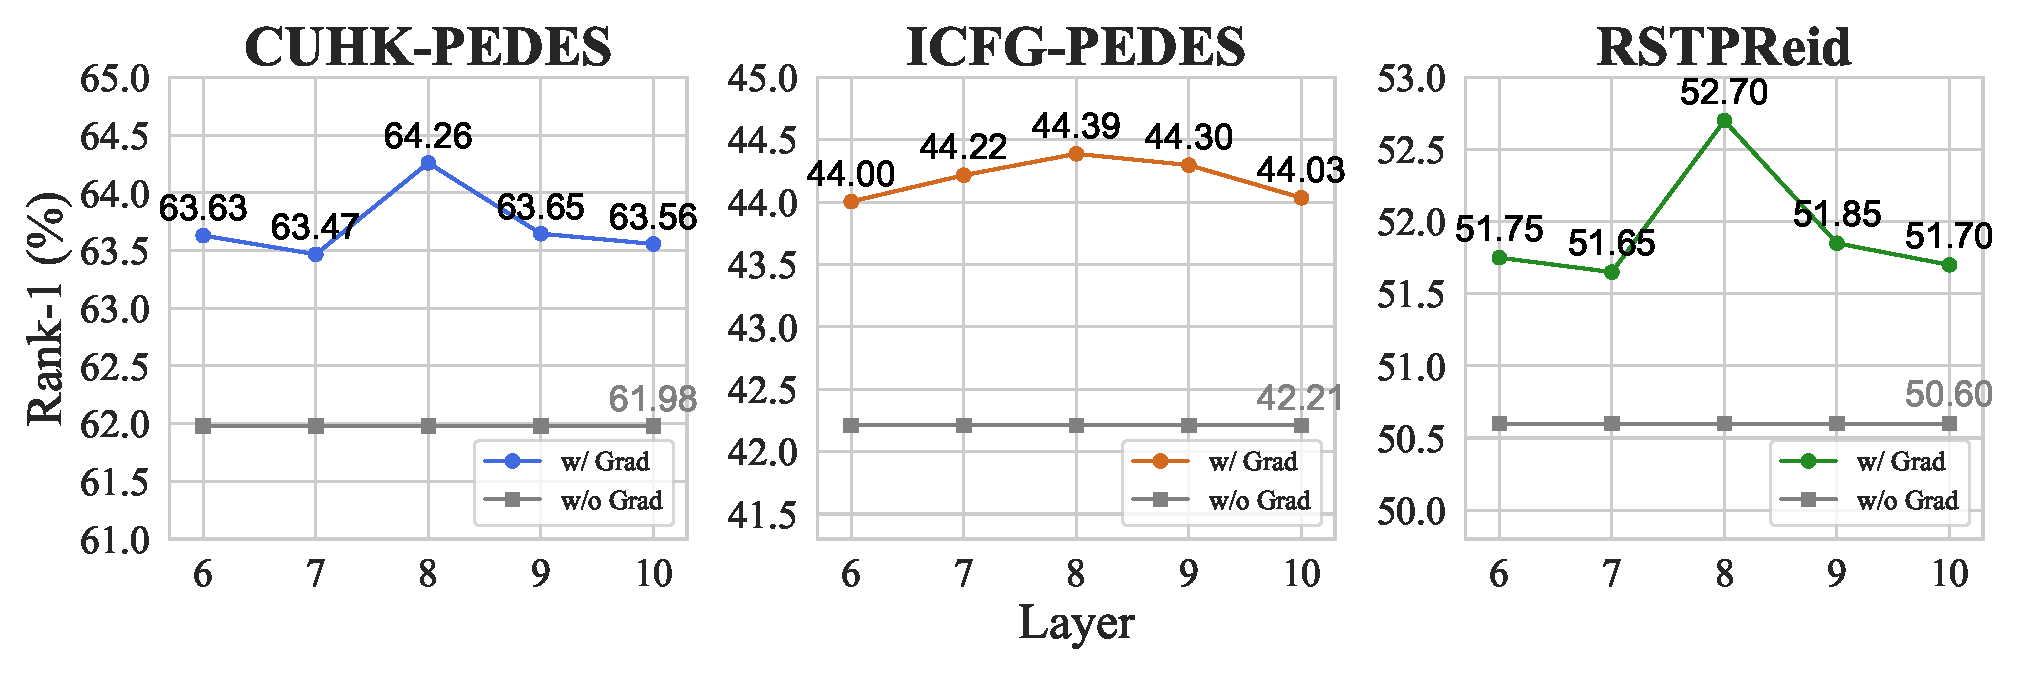
\includegraphics[width=1.0\linewidth]{Figure/Layer.pdf}}
\vspace{-2mm}
  \caption{Results of different layers to compute $\mathbb{S}$. The encoders contain 12 layers in total.}
  \label{fig:layer}
  \vspace{-5mm}
\end{figure}

\begin{table*}[t!]
\centering

\label{table:dataset}
\resizebox{0.95\linewidth}{!}{
\begin{tabular}{c|c|c|c|c|c|c}
\hline 
Datasets                  &Year &\#Images &\#Descriptions &Data Source &\#Vocabulary Size & Label Method  \\
\hline 
CUHK-PEDES~\cite{li2017person}&2017 &40,206 &80,412 &Market, Duke, etc. &12,517 &Manual \\
LPW~\cite{song2018region}            &2018 &592,438&-      &Surveillance Video                 &-  &Manual+Detector+NN\\
MSMT-17~\cite{MSMT17}     &2018 &126,441&-      &Manual Collection   &-  &FasterRCNN\\
RSTPReid~\cite{zhu2021dssl}  &2021 &20,505 &41,010  &MSMT-17             &6,331 &Manual \\
ICFG-PEDES~\cite{ding2021semantically}    &2021 &54,522 &54,522 &MSMT-17             &5,848 &Manual \\
LUPerson~\cite{fu2021unsupervised}       &2021 &4,180,243&-    &YouTube             &-  &YOLOv5 \\
LUPerson-NL~\cite{fu2022large}  &2022 &10,683,716&-   &YouTube             &-  &FairMOT\\
MALS~\cite{yang2023towards}          &2023 &1,510,330&1,510,330&Automatic Synthesis&4,772 &ImaginAIry\\
LuPerson-T~\cite{shao2023unified}&2023&957,606 &1,277,991   &LUPerson       &459 &CLIP\\
Luperson-MLLM~\cite{tan2024harnessing}&2024&1,020,022   &2,037,239   &LUPerson &39,566  &MLLM\\
SYNTH-PEDES~\cite{zuo2024plip}&2024  &4,791,771   &12,138,157  &LUPerson-NL\& LPW  &8,598  &SPAC\\
\hline
\cellcolor{gray!20}\textbf{WebPerson}&\cellcolor{gray!20}2025&\cellcolor{gray!20}5,002,723&\cellcolor{gray!20}10,005,446&\cellcolor{gray!20}COYO-700M &\cellcolor{gray!20}96,623 &\cellcolor{gray!20}MLLM \\
\hline 
\end{tabular}}
\vspace{-2mm}
\caption{Statistical comparison of different datasets. WebPerson stands as the largest automatically-generated text-described person dataset, offering inherent scalability without manual annotation requirements.}
\label{dataset}
\vspace{-3mm}
\end{table*}



\subsection{Dataset analysis}
Current text-based person retrieval datasets predominantly consist of manually annotated pedestrian images from re-identification benchmarks, fundamentally limited in scale and diversity by the substantial costs of human annotation. While generative methods have shown promise for dataset augmentation, they fail to achieve the necessary scale and fidelity for practical deployment. The emergence of Multimodal Large Language Models (MLLMs) and the availability of web-scale image resources now enable a new paradigm for automated dataset construction. Our WebPerson dataset leverages novel image filtering and text generation techniques to create a comprehensive pedestrian image library with accurate textual descriptions across diverse scenarios. Compared to existing datasets, WebPerson offers three key advantages:

\noindent{\bf High-quality} WebPerson surpasses existing datasets containing single-style synthetic images or low-quality surveillance footage by providing superior texture details and diverse scene variations. Our rigorous image filtering pipeline ensures exceptional visual fidelity, while the MLLM-powered text generation framework produces highly accurate and detailed descriptions. Fig.~\ref{visual-dataset} showcases representative examples demonstrating precise textual characterization of pedestrian attributes.


\begin{figure}[t!]
\centering
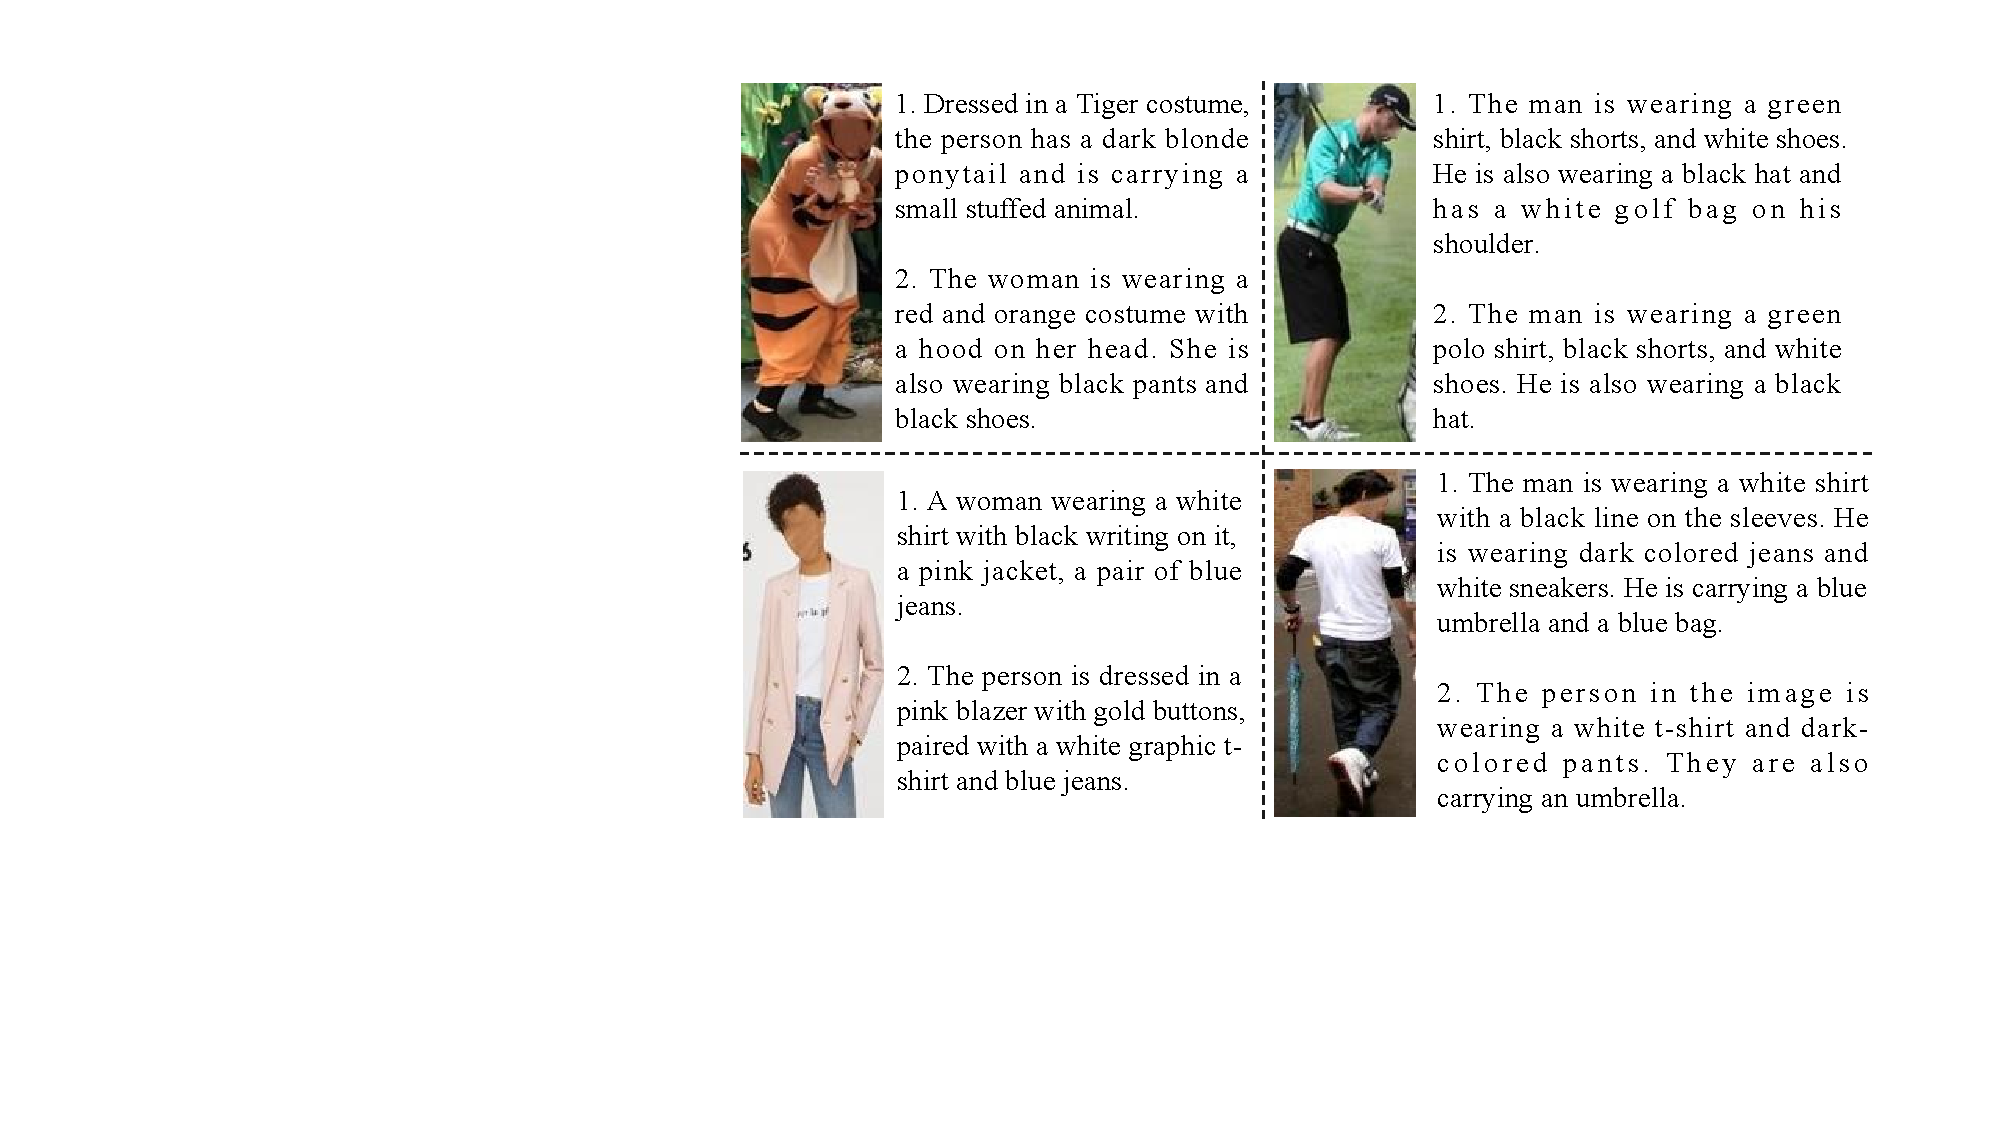
\includegraphics[width=\linewidth]{Figure/dataset-example.pdf}
\caption{Visualization of some examples in our WebPerson dataset.}

\label{visual-dataset}
\vspace{-3mm}
\end{figure}


\noindent{\bf Diversity} Sourced from web data, WebPerson exhibits rich variations in images, including but not limited to scene diversity, viewpoint changes, occlusions, clothing variations, and body poses. Our caption generation strategy further ensures corresponding textual descriptions maintain sufficient diversity. This dual-modality diversity enables WebPerson to serve as an effective training corpus for developing robust models that generalize well to novel and unseen data across visual tasks, language tasks, and vision-language tasks.

\noindent{\bf Large-scale} As illustrated in Tab.~\ref{dataset}, we compare the attributes of WebPerson with other prominent person datasets. WebPerson emerges as the most extensive real-world dataset, featuring high-quality image-text pairs, encompassing 5 million images and 10 million textual descriptions. Moreover, our efficient data collection and caption generation strategies enable seamless scalability in data volume.

\subsection{Broader Impact}
\label{broad_impact}
This work introduces a novel pedestrian representation learning framework that achieves fine-grained cross-modal alignment through gradient-based token-wise similarity scoring while effectively suppressing noise interference. Complementing this framework, we construct WebPerson, a large-scale human-centric dataset with diverse web-sourced image-text pairs. Together, these contributions demonstrate robust performance in human-oriented applications, including intelligent surveillance and autonomous retail systems.
